\documentclass[tikz,border=10pt]{standalone}
\usepackage{pgfplots}
\pgfplotsset{compat=1.18}
\usetikzlibrary{arrows.meta,positioning,calc,shapes}

\definecolor{politoNavy}{RGB}{0, 43, 91}
\definecolor{deepdiveTeal}{RGB}{0, 128, 128}
\definecolor{examred}{RGB}{180, 0, 0}
\definecolor{intuitiongreen}{RGB}{34, 139, 34}

\begin{document}
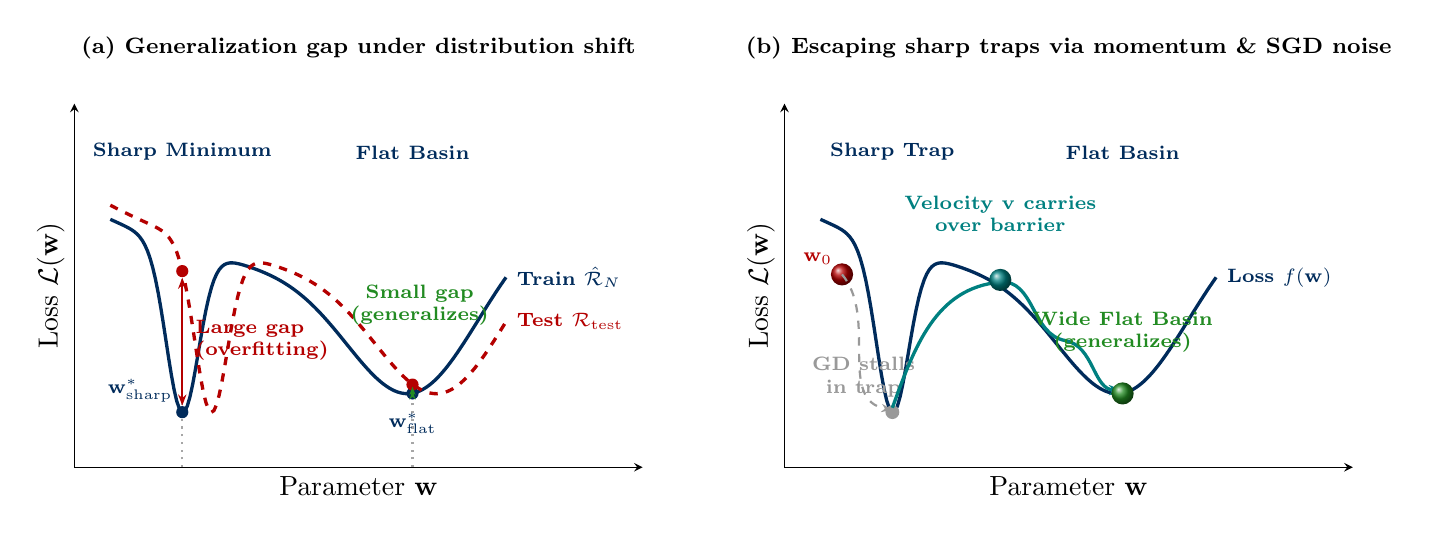
\begin{tikzpicture}
  % Panel A: Flat vs Sharp Minima under Distribution Shift
  \begin{axis}[
    name=plot1,
    width=8.8cm, height=6.2cm,
    axis lines=left,
    xlabel={Parameter $\mathbf{w}$},
    ylabel={Loss $\mathcal{L}(\mathbf{w})$},
    xmin=0.5, xmax=8.4,
    ymin=0, ymax=3.3,
    ticks=none,
    title={\textbf{(a) Generalization gap under distribution shift}},
    title style={font=\footnotesize, at={(0.5,1.05)}, anchor=south}
  ]
    % Train loss
    \addplot[very thick, politoNavy, domain=1.0:6.5, samples=150] 
      {1.8 + 0.05*(x-4.0)^2 - 1.5*exp(-(x-2.0)^2 / 0.10) - 1.2*exp(-(x-5.2)^2 / 1.5)}
      node[pos=1.0, right, font=\scriptsize\bfseries, text=politoNavy] {Train $\hat{\mathcal{R}}_N$};

    % Test loss (shifted by Delta w = 0.4)
    \addplot[very thick, examred, dashed, domain=1.0:6.5, samples=150] 
      {1.8 + 0.05*(x-0.4-4.0)^2 - 1.5*exp(-(x-0.4-2.0)^2 / 0.10) - 1.2*exp(-(x-0.4-5.2)^2 / 1.5)}
      node[pos=1.0, right, font=\scriptsize\bfseries, text=examred] {Test $\mathcal{R}_{\mathrm{test}}$};

    % Sharp minimum point at x = 2.0
    \draw[dotted, thick, gray!70] (axis cs:2.0, 0) -- (axis cs:2.0, 1.78);
    \fill[politoNavy] (axis cs:2.0, 0.50) circle (2.2pt);
    \fill[examred] (axis cs:2.0, 1.78) circle (2.2pt);
    \node[above left, font=\scriptsize\bfseries, text=politoNavy] at (axis cs:2.0, 0.50) {$\mathbf{w}^*_{\mathrm{sharp}}$};
    
    % Vertical gap at sharp minimum
    \draw[{Stealth[length=4pt]}-{Stealth[length=4pt]}, thick, examred] (axis cs:2.0, 0.56) -- (axis cs:2.0, 1.72);
    \node[right, font=\scriptsize\bfseries, text=examred, align=left] at (axis cs:2.05, 1.15) {Large gap\\(overfitting)};

    % Flat minimum point at x = 5.2
    \draw[dotted, thick, gray!70] (axis cs:5.2, 0) -- (axis cs:5.2, 0.75);
    \fill[politoNavy] (axis cs:5.2, 0.67) circle (2.2pt);
    \fill[examred] (axis cs:5.2, 0.75) circle (2.2pt);
    \node[below, font=\scriptsize\bfseries, text=politoNavy] at (axis cs:5.2, 0.58) {$\mathbf{w}^*_{\mathrm{flat}}$};

    % Small gap at flat minimum
    \draw[{Stealth[length=3pt]}-{Stealth[length=3pt]}, thick, intuitiongreen] (axis cs:5.2, 0.69) -- (axis cs:5.2, 0.73);
    \node[above, font=\scriptsize\bfseries, text=intuitiongreen, align=center] at (axis cs:5.3, 1.20) {Small gap\\(generalizes)};

    % Basin labels
    \node[above, font=\scriptsize\bfseries, text=politoNavy] at (axis cs:2.0, 2.7) {Sharp Minimum};
    \node[above, font=\scriptsize\bfseries, text=politoNavy] at (axis cs:5.2, 2.7) {Flat Basin};
  \end{axis}

  % Panel B: Escaping Sharp Traps via Momentum and Stochastic Noise
  \begin{axis}[
    name=plot2,
    at={($(plot1.east)+(1.8cm, 0)$)},
    anchor=west,
    width=8.8cm, height=6.2cm,
    axis lines=left,
    xlabel={Parameter $\mathbf{w}$},
    ylabel={Loss $\mathcal{L}(\mathbf{w})$},
    xmin=0.5, xmax=8.4,
    ymin=0, ymax=3.3,
    ticks=none,
    title={\textbf{(b) Escaping sharp traps via momentum \& SGD noise}},
    title style={font=\footnotesize, at={(0.5,1.05)}, anchor=south}
  ]
    % Loss landscape
    \addplot[very thick, politoNavy, domain=1.0:6.5, samples=150] 
      {1.8 + 0.05*(x-4.0)^2 - 1.5*exp(-(x-2.0)^2 / 0.10) - 1.2*exp(-(x-5.2)^2 / 1.5)}
      node[pos=1.0, right, font=\scriptsize\bfseries, text=politoNavy] {Loss $f(\mathbf{w})$};

    % Initial point w0
    \coordinate (w0) at (axis cs:1.3, 1.75);
    \shade[ball color=examred] (w0) circle (4pt) node[above left, font=\scriptsize\bfseries, text=examred] {$\mathbf{w}_0$};

    % GD path into sharp trap
    \draw[-{Stealth[length=4pt]}, thick, gray!80, dashed] (w0) to[out=-50, in=170] (axis cs:2.0, 0.52);
    \fill[gray!80] (axis cs:2.0, 0.50) circle (2.5pt);
    \node[above, font=\scriptsize\bfseries, text=gray!80, align=center] at (axis cs:1.6, 0.55) {GD stalls\\in trap};

    % Momentum trajectory flowing along the curve and overcoming barrier
    \draw[-{Stealth[length=5pt]}, very thick, deepdiveTeal] (axis cs:2.0, 0.54) 
      to[out=70, in=185] (axis cs:3.5, 1.68)
      to[out=5, in=170] (axis cs:4.4, 1.15)
      to[out=-10, in=180] (axis cs:5.2, 0.70);
    
    % Ball at the barrier
    \shade[ball color=deepdiveTeal] (axis cs:3.5, 1.70) circle (4pt);
    \node[above, font=\scriptsize\bfseries, text=deepdiveTeal, align=center] at (axis cs:3.5, 2.05) {Velocity $\mathbf{v}$ carries\\over barrier};

    % Ball in flat basin
    \shade[ball color=intuitiongreen] (axis cs:5.2, 0.67) circle (4pt);
    \node[above, font=\scriptsize\bfseries, text=intuitiongreen, align=center] at (axis cs:5.2, 0.95) {Wide Flat Basin\\(generalizes)};

    % Basin labels
    \node[above, font=\scriptsize\bfseries, text=politoNavy] at (axis cs:2.0, 2.7) {Sharp Trap};
    \node[above, font=\scriptsize\bfseries, text=politoNavy] at (axis cs:5.2, 2.7) {Flat Basin};
  \end{axis}
\end{tikzpicture}
\end{document}
